\section{Measured results}
\label{sec:results}
The following numbers are measurements of this study. The new test holds the exact identities and the selected model fixed. Table~\ref{tab:light-results} separates the physical groups and retains incomplete controls. A completed request must agree with its reference in every repetition.
\begin{table}[!htbp]\centering\small
\caption{Complete application times against the preceding application. Done gives preceding/new completions; times sum request medians on the matched completed subset only. A dash means no matched pair.}
\label{tab:light-results}
\begin{tabularx}{\linewidth}{@{}Yrrrr@{}}\toprule
Requests & Done & Paired & Preceding (s) & New (s)\\\midrule
Zero-invariant tensor bubbles & 20/20 & 20 & 27.055 & 5.856 \\
Symbolic scalar masses & 3/3 & 3 & 4.564 & 3.958 \\
Independent products, 2--13 loops & 12/12 & 12 & 18.818 & 2.775 \\
Larger sectors with a zero-invariant sub-sector & 3/3 & 3 & 4.856 & 0.608 \\
Ordinary one-loop tensors & 3/3 & 3 & 0.682 & 0.708 \\
Connected vacuum checks & 3/3 & 3 & 0.586 & 1.593 \\
Native two-loop box batches & 24/24 & 24 & 196.362 & 198.313 \\
All 68 requests & 68/68 & 68 & 252.923 & 213.813 \\\bottomrule\end{tabularx}\end{table}

The new application completes 68 of 68 requests, compared with 68 for the preceding application. The comparison contains 12,978 exact coefficient checks across the timed outputs. There are 0 requests without a successful external reference. On the 68 matched requests, summed median time changes from 252.923 to 213.813 seconds, a time ratio of 0.845, or 15.5\% less time. This decrease is incremental relative to the preceding implementation on the same new requests. It is not a comparison with unmodified Kira, and percentages from earlier workloads cannot be added to it. The new application is slower on 26 matched requests. These totals describe this finite collection and include native requests where the exact extension does not apply.

\subsection{Exact identities and their integration}
The new exact domains comprise 38 requests: zero-invariant tensor bubbles, symbolic scalar masses, independent products, and embedded sub-sectors. The new method completes 38 and the preceding method completes 38. Their 38 matched requests take 55.293 and 13.197 seconds, respectively. The exact rules supply the change in this comparison; no learned action is required for these recognized inputs.

Development verifies the seven direct-formula cases against Kira, checks signed IBP residuals, and compares 60 symbolic-mass coefficients after rational substitutions. The larger-sector development check compares 36 coefficients with Kira. In the reserved test, 3 of the three embedded-sector requests complete. This checks that a formula used inside a recurrence produces the same physical reduction as native elimination.

\begin{figure}[!htbp]\centering
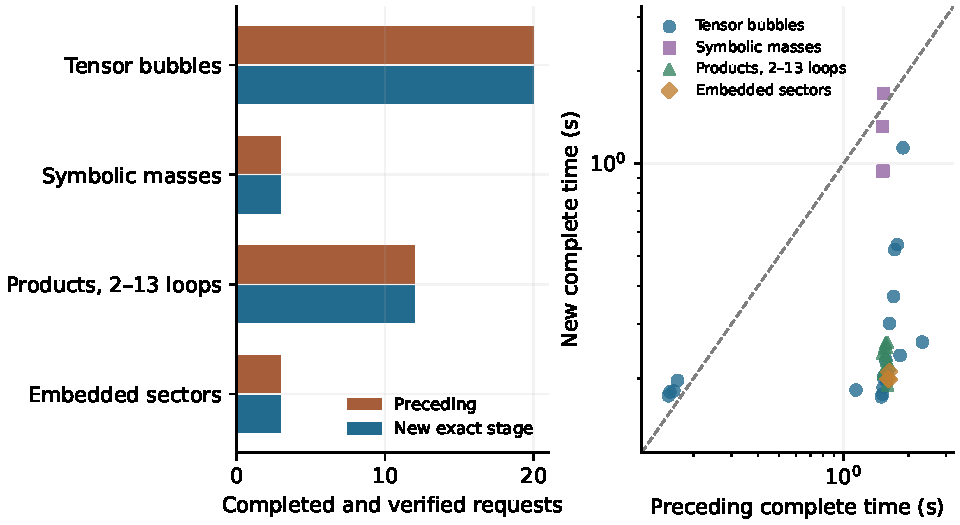
\includegraphics[width=\linewidth]{paper_figures/lightlike_exact.pdf}
\caption{Exact-extension results. The left panel compares completion counts, including failures. The right panel shows paired request times on logarithmic axes; points below the equal-time line favor the new method. Only completed, verified pairs appear in the time panel.}
\label{fig:light-exact}
\end{figure}
\subsection{The added native ML choice}
Validation selects 1 cost tree with maximum depth 2, minimum leaf population 2, a saving margin of 0\%, and a failure score threshold of 0.15. It enables the new model. The selected validation cost, including the prediction allowance and any failure penalties, is 105.848 seconds; the fixed choice gives 107.356 seconds. The selected fixed region is tight. These values determine deployment before the reserved test.

In the 24 reserved native batches, the integrated method uses the new model on 24 requests in the final repetition. Against the fixed-choice application, it completes 24 requests while the control completes 24. The 24 matched batches take 200.983 seconds with the fixed choice and 198.313 seconds with the integrated choice. The ratio is 0.987, with a central 95\% request-resampling interval of $[0.970,1.002]$. It is slower on 11 matched batches. The interval includes equal time, so this sample does not resolve a consistent additional saving. The exact formulas and native reduction interface are shared by these two controls. The learned failure check redirects predicted risky actions and inputs outside the new feature range to the verified fixed choice.

Across the 72 native applications per method, the integrated method has 0 unverified applications, the fixed control has 0, and the preceding application has 0. In the final repetition, the recorded rejection counts are 1 for predicted failure risk and 10 for inputs outside the training feature range. These checks occur before the selected native reduction. The measured failure counts, rather than a zero predicted risk, determine whether failures were avoided in this test.

The learned policy changes the fixed action on 1 of the 24 native requests in the final repetition. Its median measured loading and decision time is 3.877 milliseconds. The saved final-repetition outputs give failed inner-attempt counts of 1 for the integrated method, 2 for the fixed control, and 0 for the preceding method. Interrupted outputs can lack inner-attempt records and remain in the separate application-failure counts. Inner attempts from the first two repetitions are not retained, so these inner-attempt counts refer only to the last repetition.

Against the preceding native application, the 24 matched batches change from 196.362 to 198.313 seconds. This comparison measures the change in the deployed policy, while the fixed control measures learned selection against one preselected region. Neither comparison measures a new elimination-row policy.

\begin{figure}[!htbp]\centering
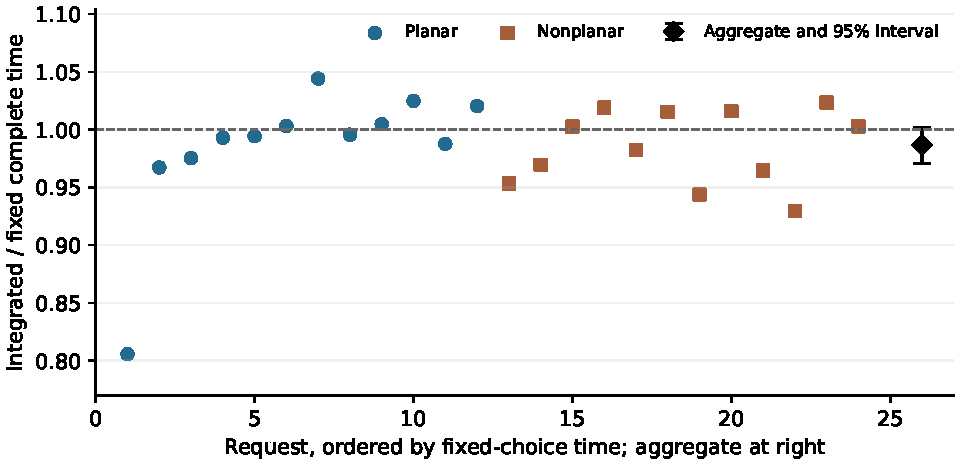
\includegraphics[width=.96\linewidth]{paper_figures/lightlike_native.pdf}
\caption{The native learned-choice comparison holds exact formulas and the native reduction interface fixed. Each point divides a request's integrated median time by its fixed-choice median. The horizontal line marks equal time. The aggregate ratio and its request-resampling interval appear separately; individual points show the observed variation across batches.}
\label{fig:light-native}
\end{figure}
\subsection{The other learned interventions}
Table~\ref{tab:retained-results} retains the main earlier controls needed to interpret the method. They use different workloads and cannot be multiplied into a cumulative speed factor. The equation-filter result supports that intervention on its tested domain, while the row results motivate its omission. The current combined experiment keeps equation filtering off and does not claim a joint seed-plus-equation gain.
\begin{table}[!htbp]\centering\small
\caption{Earlier measurements from this study, retained as separate evidence. A ratio below one means less time. Their full input definitions and measurements remain in the notes.}
\label{tab:retained-results}
\begin{tabularx}{\linewidth}{@{}YYr@{}}\toprule
Intervention & Control and workload & Time ratio\\\midrule
Earlier native seed model & Fixed region, 32 box batches: 156.383 to 150.663 s & 0.963\\
Equation selection & Native filter, 24 new-index batches: 72.295 to 67.478 s & 0.933\\
Original learned row model & Native row choices, 84 trials & 1.305\\
Compiled row-cost policy & Native row choices; geometric mean & 0.982\\\bottomrule
\end{tabularx}
\end{table}
The earlier seed comparison has interval $[0.937,0.984]$, and the equation comparison has interval $[0.928,0.940]$. The compiled row policy has interval $[0.959,1.003]$, which includes equal time. These intervals use the resampling procedure recorded for each original study. The native row algorithm remains in the retained workflow.

\subsection{Scope of the result}
The new exact identities cover their stated masses, powers, and kinematics, and the reserved comparison tests concrete instances of those identities. The independent products reach thirteen loops by factorization, while the connected vacuum checks use a one-scale tree. General coupled multiscale scattering at every loop order remains outside this evidence. The native build also has a finite integral-coordinate limit, documented in the notes; a loop count alone does not determine whether an arbitrary family can be reduced.

The learned test uses two graph types already represented during training, with new whole target batches and kinematic points. It does not establish transfer to every topology. The application keeps exact algebra and bounded recovery for supported native inputs, but neither a finite training search nor the present timings prove globally minimal reduction time. The practical result is a tested extension of the exact domain together with a separately measured policy for the remaining native work.
\FloatBarrier
